\chapter{Wing Lift Characteristics}
\label{ch:worklift}
\markboth{Wing Lift Characteristics}{}

\begin{flushright}
	{\smaller
		\textit{C'è qualcuno che può rompere il muro del suono,\\ mentre tutto il mondo si commenta da solo.}\\
		-- L. Ligabue}
\end{flushright}


Any body in motion in a fluid presents a result of force acting on it, which can be decomposed in two components:
\begin{itemize}
\item A {\bfseries Lift} acting normal to the Velocity direction and is positive upward.
\item A {\bfseries Drag} acting in the opposite direction to the airspeed vector.
\end{itemize}
The lifting surfaces of an airplane are designed to generate lift exceeding their drag, in order to obtain a positive efficiency. \\ In this chapter it will be explained how it's possible to evaluate the complete lift coefficient curve of a wing, both in its linear trait and non linear.\\
The lift coefficient is a dimensionless number used to model all of the complex dependencies of shape, inclination, and some flow conditions on lift. The lift coefficient also contains the effects of air viscosity and compressibility that are molded respectively with the Raynolds and Mach number.% [ Cap. \cite{nasaLift}] 

\section{Theoretical background}

In order to achieve the complete curve of coefficient list it's necessary to obtain the following parameters:

\begin{enumerate}
\item Zero-Lift Angle
\item Lift Coefficient slope 
\item End of Linearity Angle
\item Maximum Lift Coefficient
\item Stall Angle of attack
\end{enumerate}

Following it will be explain the theory behind how these contributions have been made.

\subsection{Zero-Lift Angle and Lift Coefficient Slope}

In order to evaluate the linear trait of the wing lift curve, it's been used the Nasa-Blackwell method.\\ The {\bfseries Nasa-Blackwell} is a numerical method for calculating the subsonic load distribution for arbitrary lifting surface arrangements at a fixed angle of attack. The method is suitable for swept wings, non-planar wings, wing with pylons and/or end-plates; it can be also used to study the aerodynamic interaction of the wing and the horizontal tail. The method has been implemented because its results, as shown in the report, were in good agreement with the experimental results.
The lifting surfaces are divided in several rectangular horse-shoe vortices along the span; one horseshoe vortex along the chord is used, that is, the midpoints of the vortices are placed only at points along the quarter-chord lines. An equal number of control points are located along the three-quarter-chord lines. The velocity from the total vortex system is equated to the component of free-stream velocity normal to the lifting surface chord at each control point. Application of this tangent-flow boundary condition for a symmetrical loading provides a set of N simultaneous equations in the N unknown circulation strengths. Solution of this set of equations provides the loading distributions over the lifting surfaces. Mach number effect is introduced through a Prandtl-Glauert correction. Further details can be found in \cite{NASA:Blackwell}.

In this way it's calculated the Zero Lift angle using the integral of the load distribution and the linear trait slope starting from the value of CL at $\alpha =  0^{\circ}$ and $\alpha = 2^{\circ}$.

\begin{equation}
CL_{\alpha}= \frac{CL|_2 - CL|_0}{\upDelta \alpha}
\end{equation}

In JPAD it is possible also evaluating these two contributes using different methods. \\
For the evaluation of the $\alpha_{0L}$ it's possible to use a method of the class \texttt{CalcAlpha0L}, a nested class  in \texttt{LSAerodynamicManager}. Using these method, the zero-lift angle is calculated with the following formula, where $\epsilon_T$ is the twist angle:

\begin{equation}
\alpha_{0L} = \frac{1}{S}\int_{-\frac{b}{2}}^{\frac{b}{2}} c(y) [ \alpha_0(y) - \epsilon_T(y) ] \, dy
\end{equation}

This formula  is applied to the exposed wing. When a default aricraft is defined, during the creation of components, is calculated the exposed wing. This is the wing outside of the fuselage. It starts at semi-diameter of fuselage and its root airfoil is the airfoil of wing  at this station calculated by the method \texttt{calculateIntermediateAirfoil}.\\ \\

In order to evaluate the lift coefficient linear slope  it's possible to use different method belonging to \texttt{CalcCLAlpha} class. The first one use the Polhamus formula which is valid for arbitrary aspect ratios and sweep angles in subsonic flow:

\begin{equation}
CL_{\alpha} = \frac{2 \pi \AR}{ \left\{ 2 + \sqrt{\frac{\AR^2 \beta^2}{k^2} \left ( 1 + \frac{\tan^2{(\Lambda_{\frac{c}{2}})}}{\beta^2} \right) + 4 }\right\}}
\end{equation}

Thus $CL_{\alpha}$  is a function of wing aspect ratio, mid-chord sweep angle $\Lambda_{\frac{c}{2}}$, Mach number, and airfoil section (defined parallel to the free stream) lift curve slope. The factor K in the equation is the ratio of the experimental two-dimensional lift curve slope.\\
Alternately it's possible to use the Anderson formula for swept wing, compressible and subsonic flow:

\begin{equation}
CL_{\alpha} = 
\frac{Cl_{\alpha} \cos{\Lambda_{\frac{c}{2}}}}
{\sqrt{1 - M^2  cos^2 {\Lambda_{\frac{c}{2}}}
 + \left[ \frac{Cl_{\alpha} \cos{\Lambda_{\frac{c}{2}}}}{\pi \AR}\right]^2} + \frac{Cl_{\alpha} \cos{\Lambda_{\frac{c}{2}}}}{\pi \AR}}
\end{equation}



\subsection{End of Linearity angle of attack}

The angle of end linearity is calculated using the characteristics of the mean airfoil of the wing. This is obtained through the influence area of the airfoils as shown in fig. \ref{fig:influencearea}.

\begin{figure}[H]
\centering
{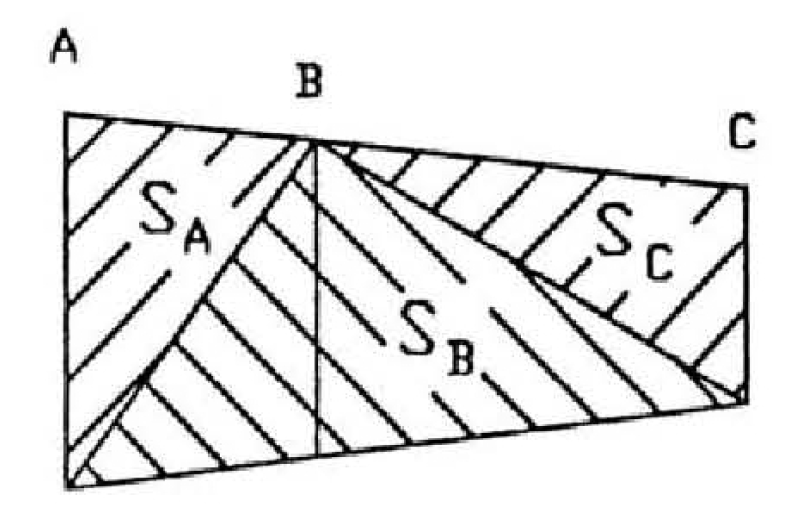
\includegraphics[height=3cm]{Immagini/influencearea}} 
\caption{Influence area of the sections for finite wing.}
\label{fig:influencearea}
\end{figure}

Then is possible to calculate the influence coefficients. 

\begin{equation}
K_i = \frac{2 S_i}{S}
\end{equation}

The mean parameters can be obtained from:

\begin{equation}
\overline{x} = x_1 K_1 + x_2 k_2 +x_3 k_3...
\end{equation}

In particular, for a wing defined by three airfoils, the end of linearity angle of attack is obtained from the following equation:

\begin{equation}
\alpha^* = \alpha^*_{1} K_1 + \alpha^*_{2} k_2 +\alpha^*_{3} k_3
\end{equation}

\subsection{Maximum Lift Coefficient}

In order to estimate the maximum lift coefficient for a clean wing it's been used the Nasa-Blackwell method. %With this method is evaluated the lift distribution of a wing and the lift coefficient through an integral. 

\begin{figure}[H]
\centering
{\includegraphics[height=6cm]{Immagini/Loading_Stall_Path_A}} 
\caption{Determination of wing lift distribution and Cl distribution of airfoils.}
\label{fig:stall0}
\end{figure}




The  practiced procedure is the following:

\begin{enumerate}
\item For each value of an Alpha array the load distribution is calculated using the NasaBlack method.  The distribution of  $Cl_{max}$ is known. fig. \ref{fig:stall1}.
\item At $\alpha = \alpha_j$ the load distribution curve intersects for the first time the $Cl_{max}$ curve of the airfoils. fig. \ref{fig:stall1}.
\item For each $ y > y_1 $ , along y axis (where y_1 is the station of first intersection) is evaluated the difference between $CL_{wing}$ and $Cl_{max}$. fig. \ref{fig:stall2}.
\item $\upDelta \alpha$ is evaluated until the maximum difference between $CL_{wing}$ and $Cl_{max}$ is smaller than the required accuracy. Actually the accuracy is 0.0001. 
\end{enumerate}

The evauation of $\upDelta \alpha$ is not simple.\\
After finding the first value of intersection between $CL_{wing}$ and $Cl_{max}$ a new $\alpha$ is evaluated. The first value used for the optimization is 

\begin{equation}\notag
\upDelta \alpha = \alpha_j -\alpha_{j-1}
\end{equation}
\begin{equation}\notag
\alpha_{new} = \alpha_j - \frac {\upDelta \alpha }{2}
\end{equation}
\begin{equation}\notag
\alpha_{old}= \alpha_j
\end{equation}

For the following step if there isn't a point of intersectionat $\alpha_{new}$ the new value of $\alpha$ is, for the step $j+1$:


\begin{equation}\notag
\upDelta \alpha = |\alpha_{j-1} -\alpha_{j}|
\end{equation}
\begin{equation}\notag
\alpha_{new} = \alpha_{j} + \frac {\upDelta \alpha }{2}
\end{equation}
\begin{equation}\notag
\alpha_{old}= \alpha_j
\end{equation}

Instead,  if there is a point of intersectionat $\alpha_{new}$ the new value of $\alpha$ is, for the step $j+1$:


\begin{equation}\notag
\upDelta \alpha =  |\alpha_{j-1} -\alpha_{j}|
\end{equation}
\begin{equation}\notag
\alpha_{new} = \alpha_{j} - \frac {\upDelta \alpha }{2}
\end{equation}
\begin{equation}\notag
\alpha_{old} = \alpha_j
\end{equation}



\begin{figure}[H]
\centering
{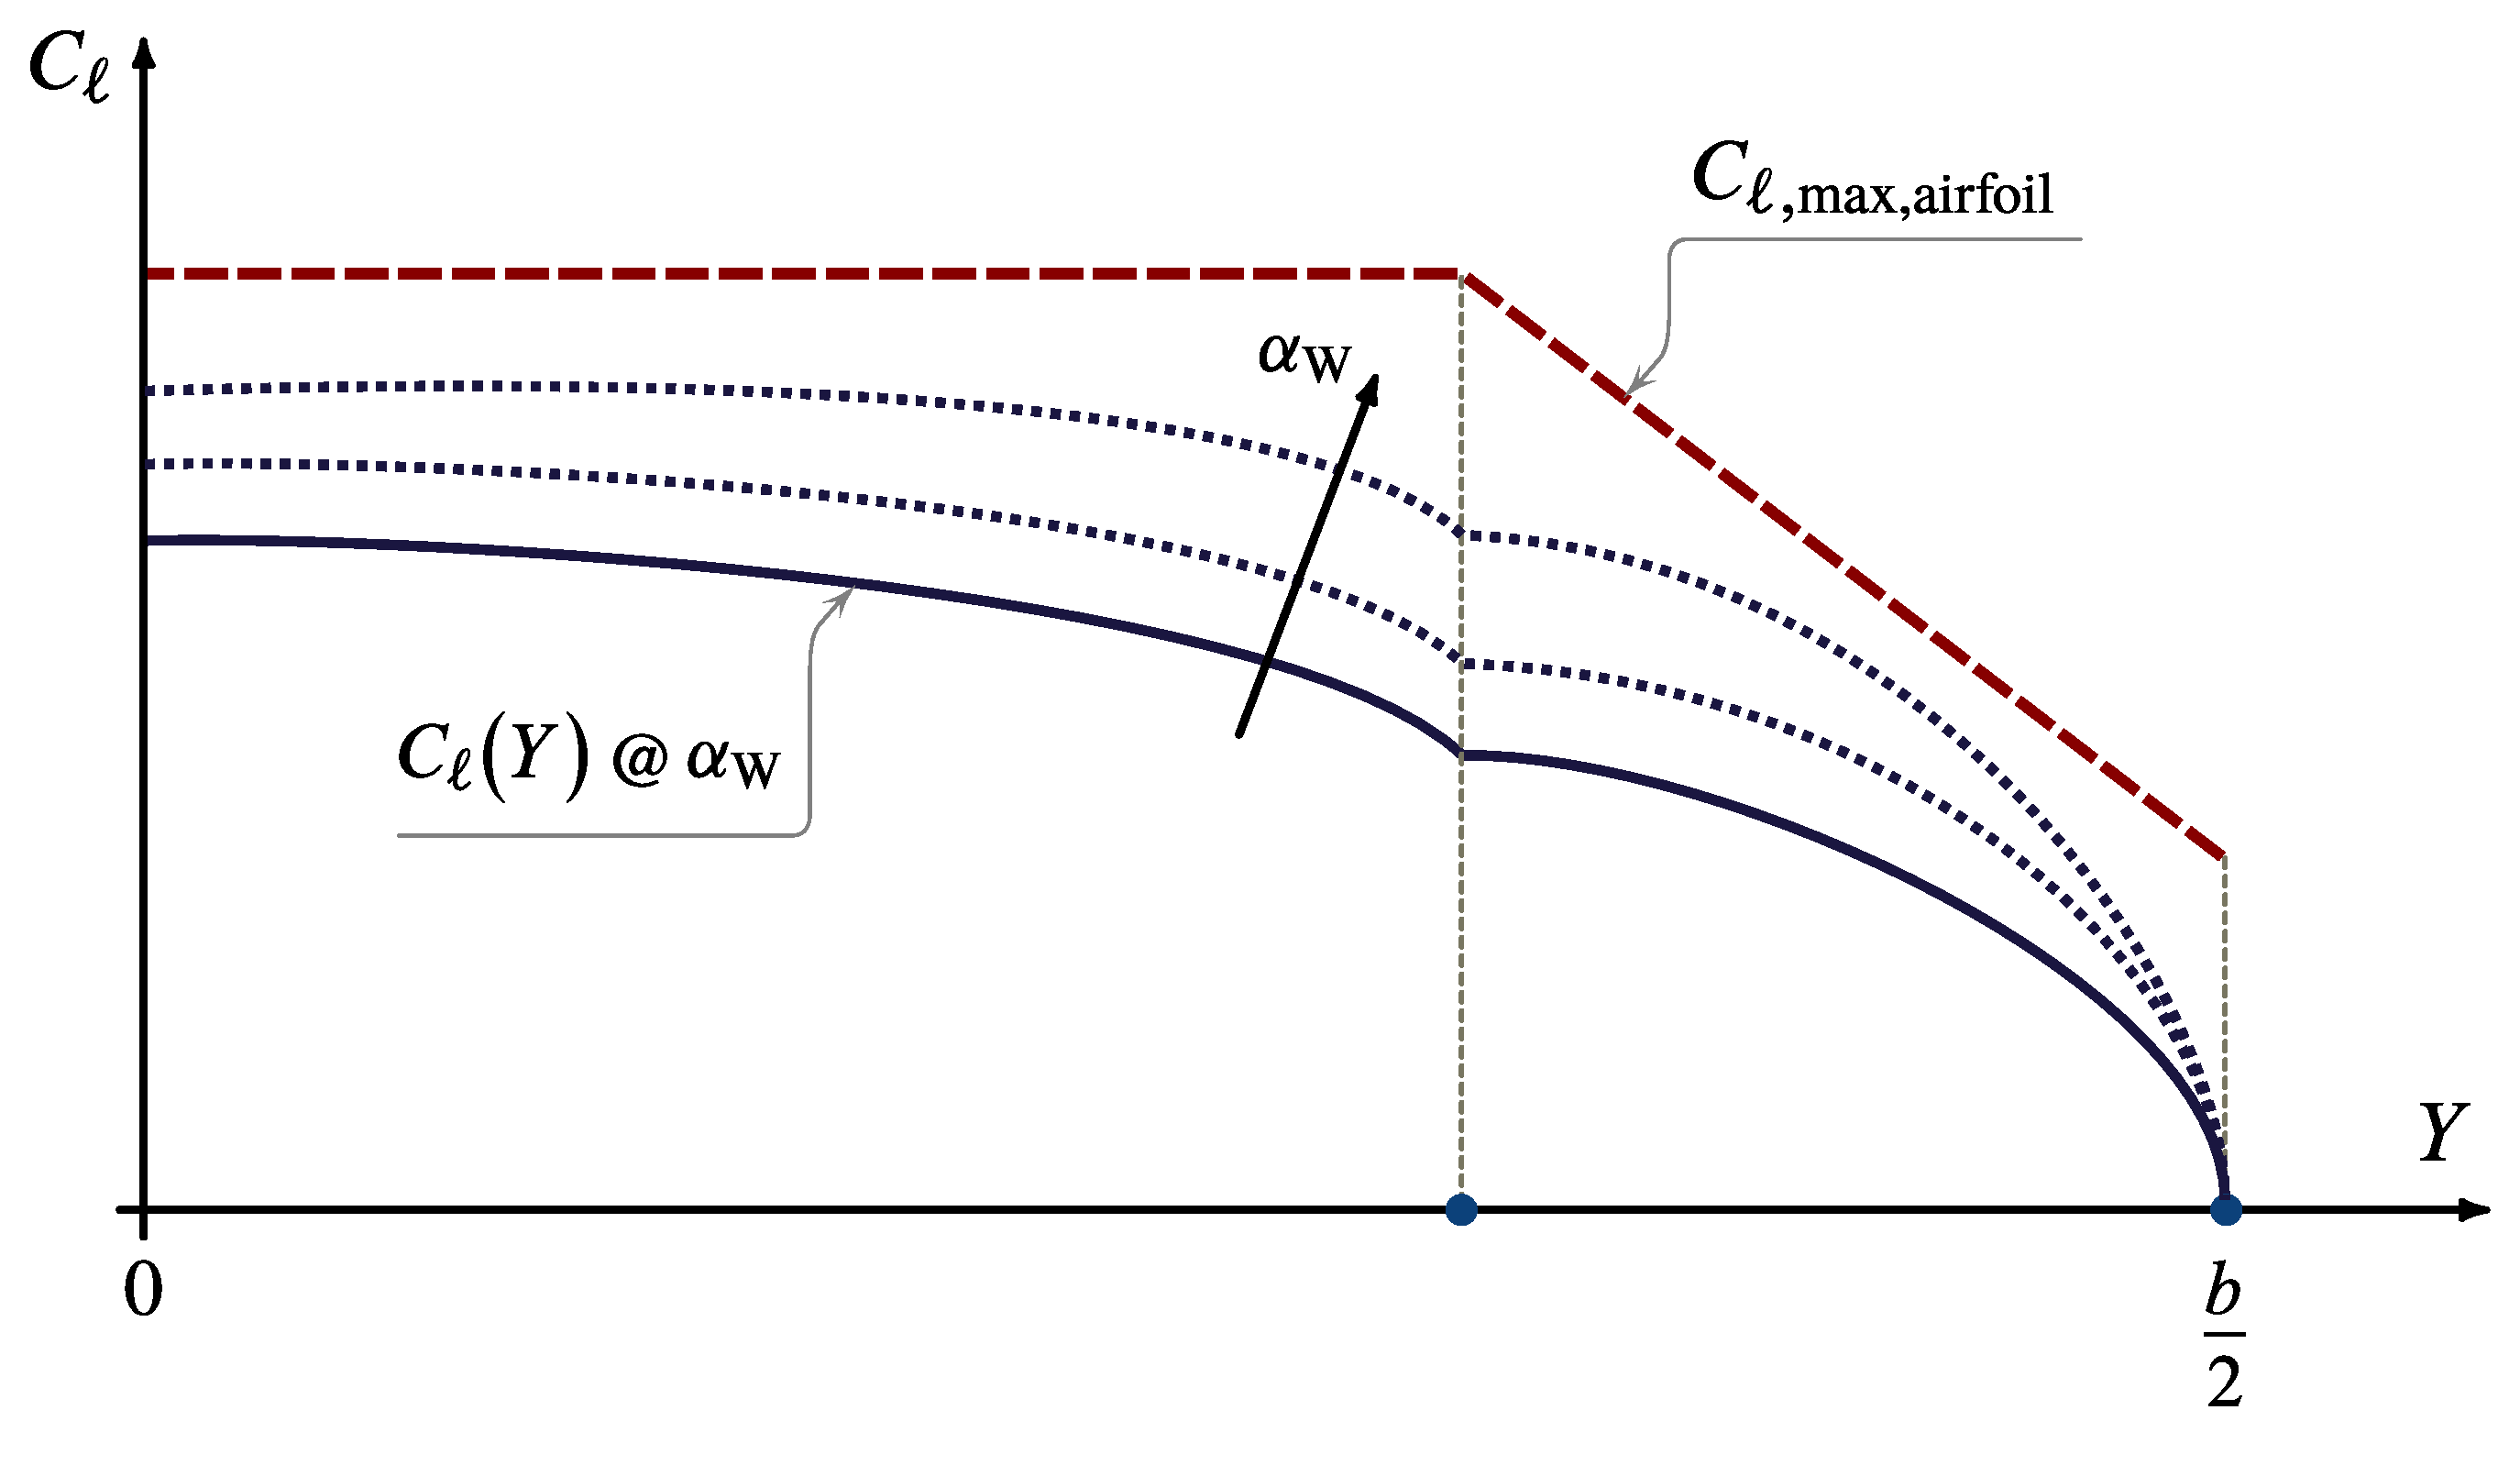
\includegraphics[height=6cm]{Immagini/Loading_Stall_Path_B}} 
\caption{Determination of wing lift distribution and Cl distribution of airfoils.}
\label{fig:stall1}
\end{figure}


\begin{figure}[H]
\centering
{\includegraphics[height=6cm]{Immagini/Loading_Stall_Path_D}} 
\caption{Intersection  between $CL_{wing}$ and $Cl_{max}$ curves.}
\label{fig:stall2}
\end{figure}

\begin{figure}[H]
\centering
{\includegraphics[height=6cm]{Immagini/Loading_Stall_Path_E}} 
\caption{Determination of $\upDelta \alpha$.}
\label{fig:stall5}
\end{figure}

\begin{figure}[H]
\centering
{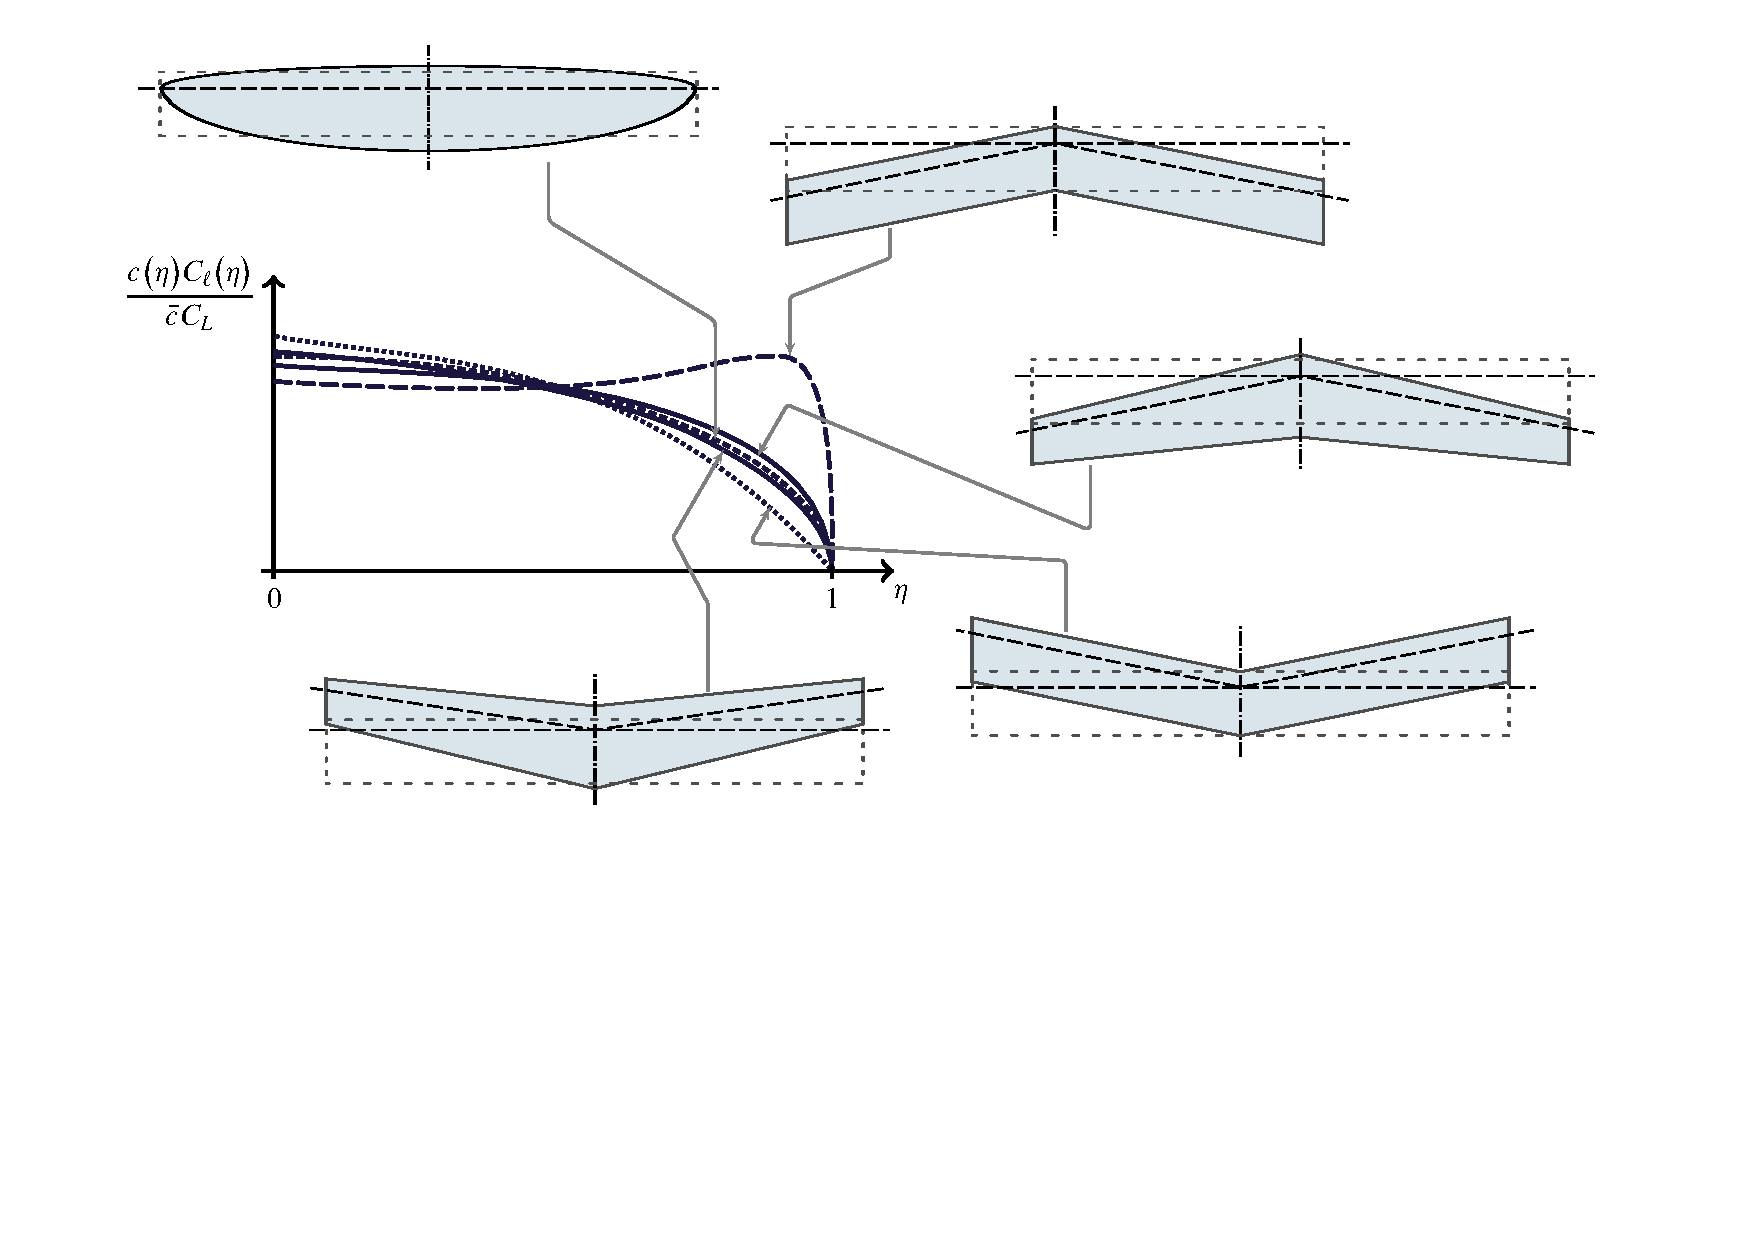
\includegraphics[height=8.3cm]{Immagini/wing_loading_B}} 
\caption{Wing Loading distribution.}
\label{fig:wl}
\end{figure}

\subsection{Stall Angle of Attack}

Nasa-Blackwell is an inviscid method for calculating the subsonic aerodynamic load distributions for arbitrary lifting-surface arrangements. This means that it doesn't see the non linear trait of the lift curve. So in correspondence of the value of $C_{L_{MAX}}$ calculated, the angle of attack obtained from the Nasa-Blackwell method is not correct because it is the maximum angle of attack that you would get if you reach the max $C_L$ linearly.\\
Obtained the maximum cl is therefore necessary to calculate the $\upDelta \alpha$ from the following graph. So first it’s evaluated the angle of attack at maximum lift coefficient through the linear trend of the lift line, then it’s added to this angle the increment evaluated by the diagram in fig. \ref{fig:dealpha}. , this is valid strictly for wing with high taper ratio without twist, with unique airfoil type and Mach number included between 0.2 and 0.6.


\begin{figure}[H]
\centering
{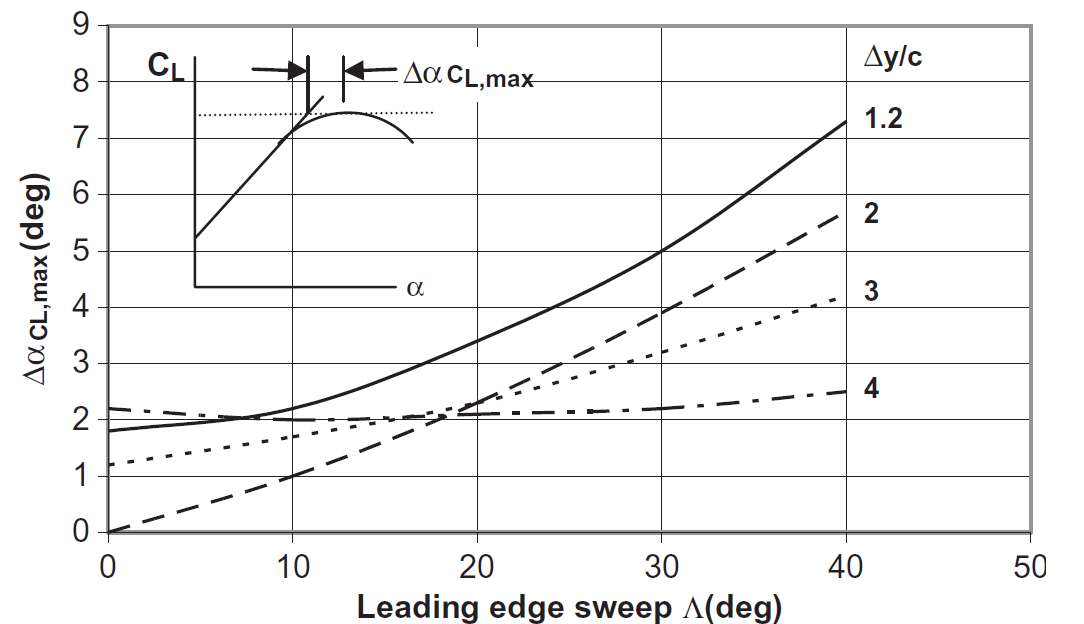
\includegraphics[height=6cm]{Immagini/deltaAlphaSforza.png}} 
\caption{Diagram useful for evaluation of $\upDelta \alpha$.}
\label{fig:dealpha}
\end{figure}



\subsection{Construction of the curve}
At this point all elements are available in order to draft the CL vs $\alpha$ curve.\\ The linear trait is evaluated using the equation of straight line.

\begin{equation}
C_L= C_{L_\alpha} \alpha + C_{L_0}
\end{equation}

%There is a method in \texttt{LSAerodynamicManager} that evaluates the linear slope of lift curve of a lifting surface using Nasa-Blackwell method. This method ( \texttt{nasaBlackwell} in the nested class\texttt{CalcCLAlpha()} evaluate CL wing in correspondence of two alpha and calculates the angolar coefficient.

In order to plot the non linear trait is used a cubic function. In fact in this zone we have four conditions:

\begin{itemize}
\item Pass to $\alpha^{\star}$ , $C_L^{\star}$
\item The derivatine in  $\alpha^{\star}$ , $C_L^{\star}$ is $C_{L_\alpha}$ for continuity
\item Pass to $\alpha_{stall}$ , $C_{L_{MAX}}$
\item The derivatine in  $\alpha_{stall}$ , $C_{L_{MAX}}$ is $0$.Here there is the maximum of the curve.
\end{itemize}

So the system of equations is :

\begin{equation}
\begin{cases}
 C_L^{\star} = a {\alpha^{\star}}^3 +  b {\alpha^{\star}}^2 +  c {\alpha^{\star}} + d \\
 C_{L_\alpha} = 3 a {\alpha^{\star}}^2 +  2b {\alpha^{\star}} +  c  \\ 
 C_{L_{MAX}} = a {\alpha_{stall}}^3 +  b {\alpha_{stall}}^2 +  c {\alpha_{stall}} + d \\
0 = 3 a {\alpha_{stall}}^2 +  2b {\alpha_{stall}} +  c  \\ 
  \end{cases}
\end{equation}



\begin{figure}[H]
\centering
{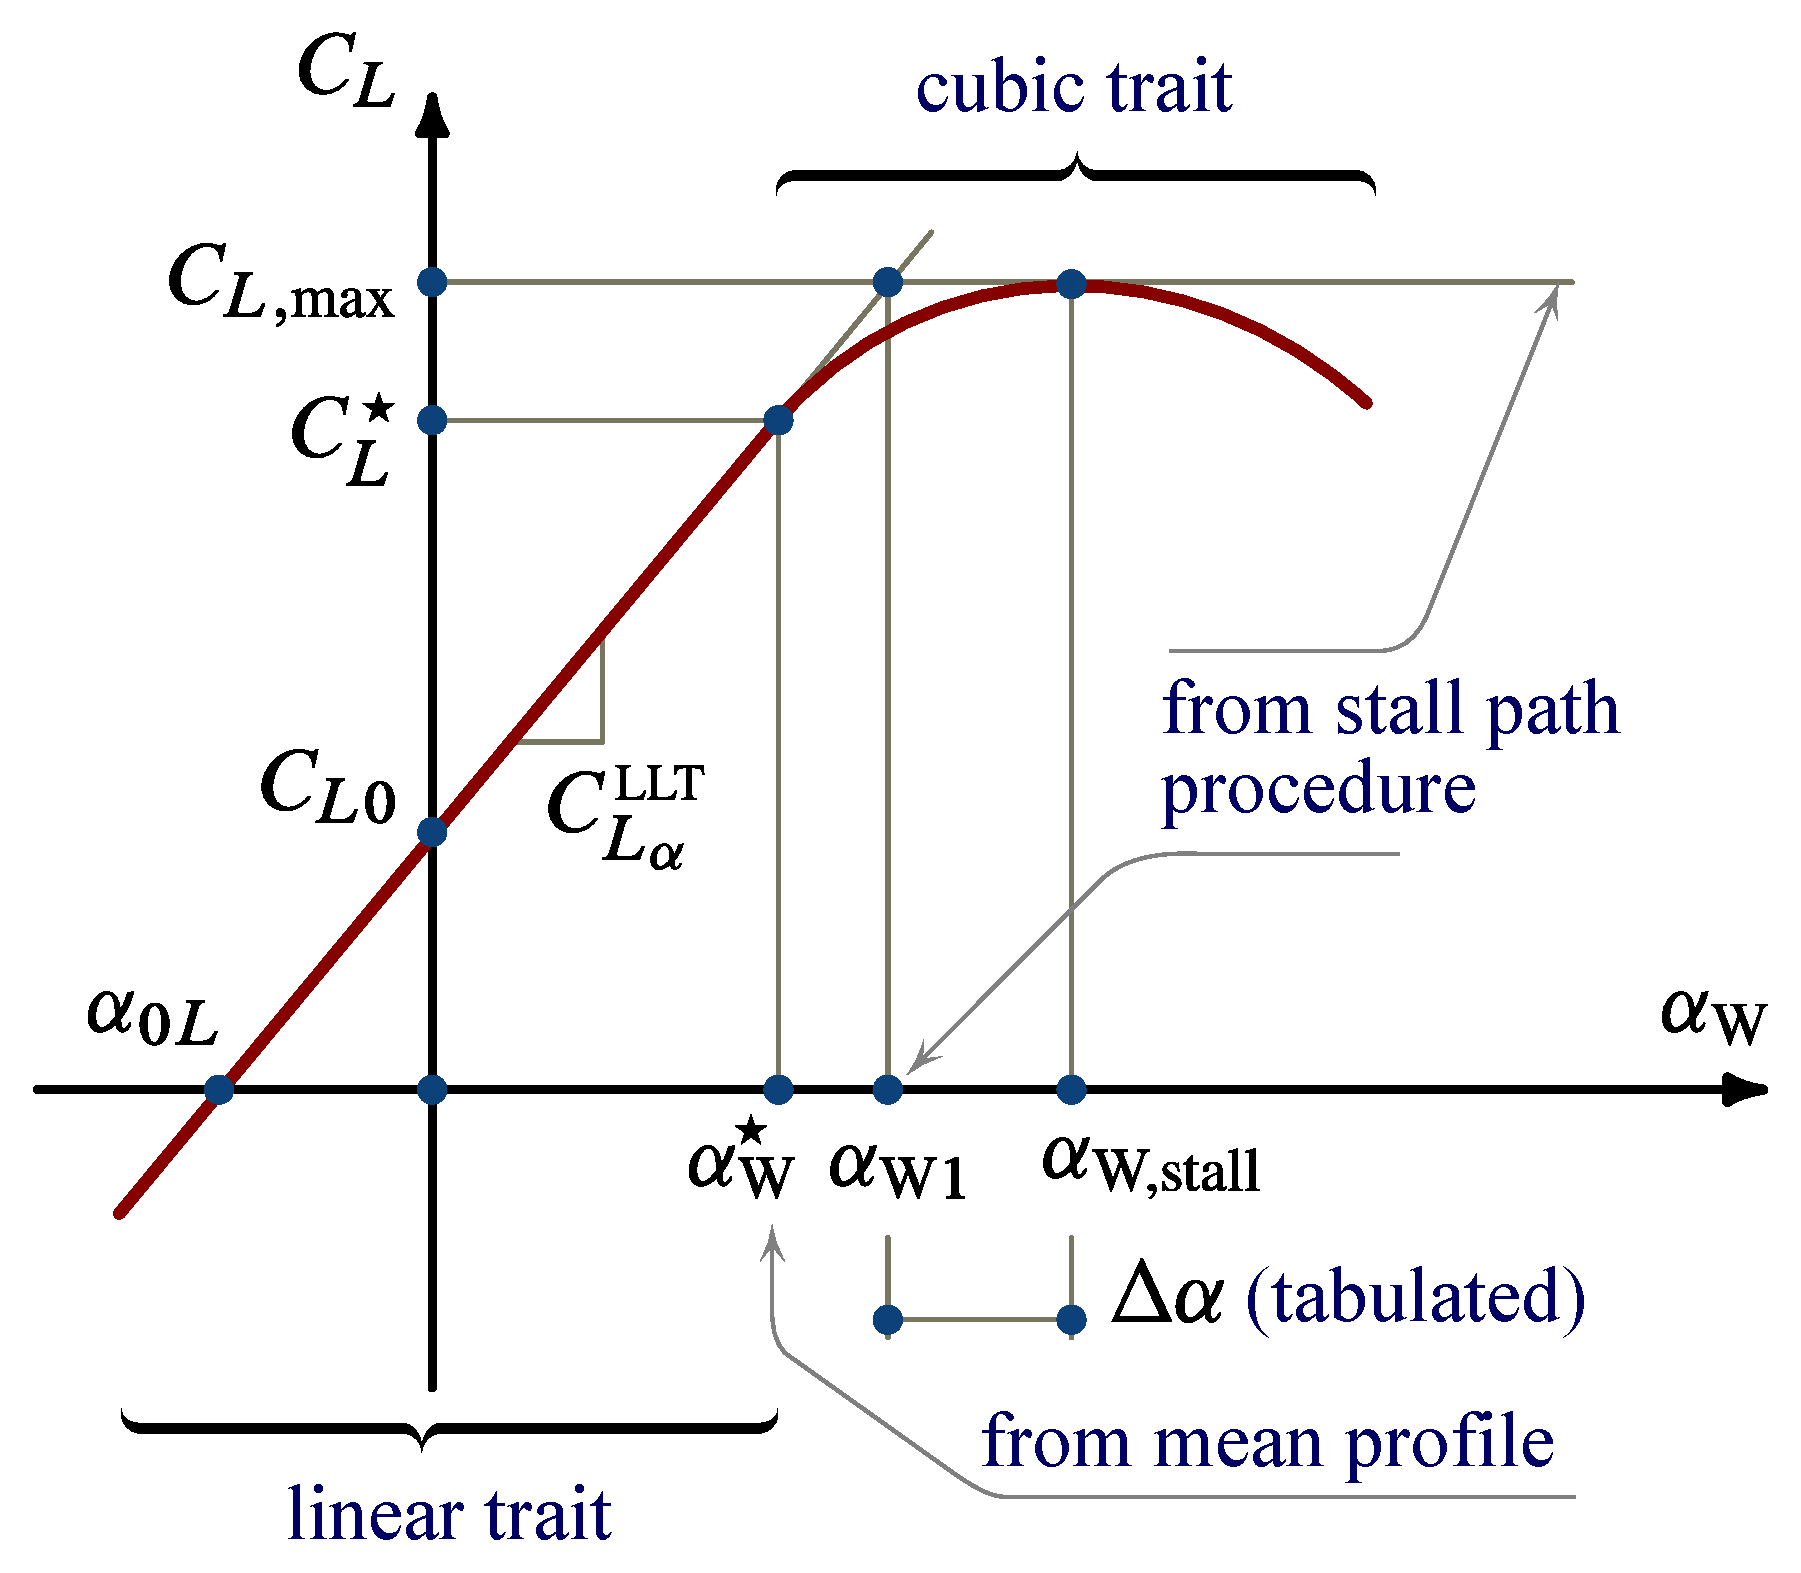
\includegraphics[height=8.69cm]{Immagini/Wing_CL_Vs_alpha_curve.pdf}} 
\caption{Wing $C_L$ vs $\alpha$ curve.}
\label{fig:clalfa}
\end{figure}


%The method that draws the curve is \texttt{plotCLvsAlphaCurve()} in \texttt{LSAerodynamicsManager}.\\
%The method \texttt{plotCLvsAlphaCurve()} solves the system and calculates the parameters using a static function of \texttt{MyMathUtils}, \texttt{solveLinearSystem}.

\subsection{Mach number effects on Lift curve }
The characteristics of airflow depend heavily from the Mach number. These changes in airflow have a significant effect on the airplane lift. For airplanes that operate entirely within the subsonic speed range, there are no significant effects of compressibility of the air on the airplane lift. For airplane that operate at high subsonic speeds in the transonic speed region, the airplane lift and drag curves will vary as the flight Mach number is increased due to the compressible nature of the air, so there is a family of lift curves one for each flight Mach number of interest.\\
The family of lift curves is characterized by an increase in the slope of the curve and decrease in maximum lift coefficient as the Mach number increased in the high subsonic region as shown in the fig. \ref{fig:clalfawing}.
The explanation of these Mach number effects on the lift curve has been derived from the theory of compressible flow, and confirmed by experimental data obtained in wind tunnels and from flight tests. It can be shown that, for an airplane at given angle of attack, the lift coefficient will increase with Mach number because the suction on the wing upper surfac, and the pressures on the wing lower surface tend to grow with Mach number.  \cite{manual}

\begin{figure}[H]
\centering
{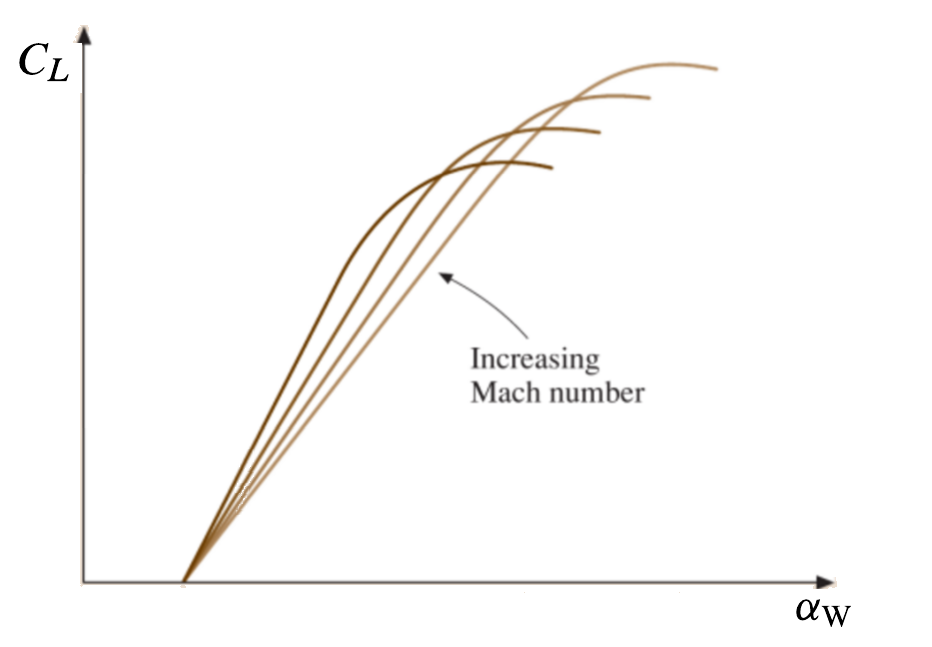
\includegraphics[height=5.6cm]{Immagini/clamach}} 
\caption{Mach number effects on Lift curve.}
\label{fig:clalfawing}
\end{figure}

\begin{figure}[H]
\centering
{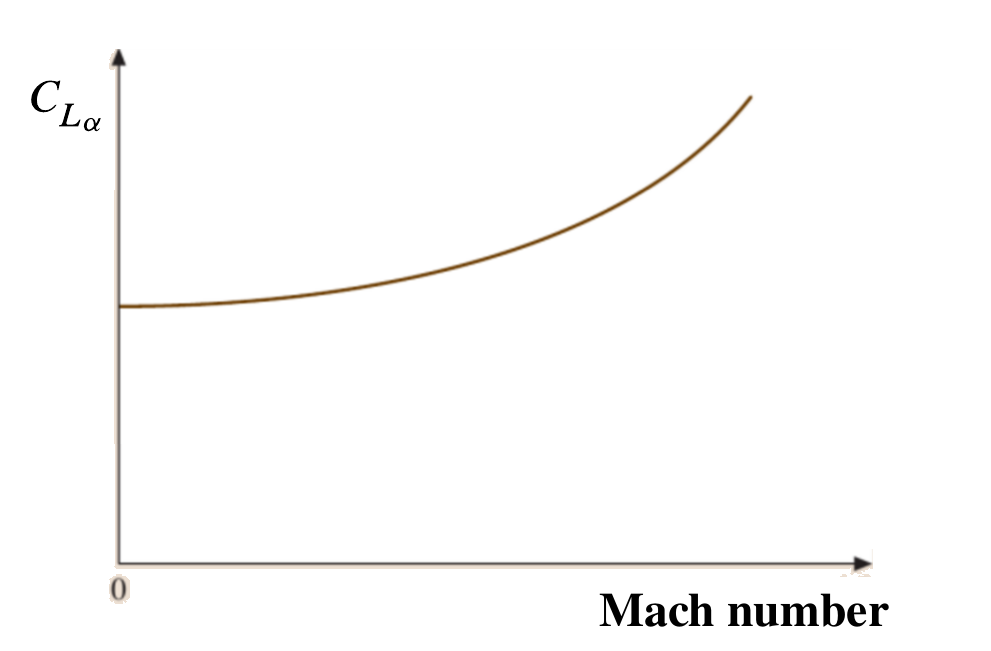
\includegraphics[height=5.6cm]{Immagini/declmach.png}} 
\caption{Mach number effects on Lift linear slope.}
\label{fig:clalfawingslope}
\end{figure}

\subsection{High Lift devices}
The aircraft’s performances at low speed are very important for their mission, infact good high lift devices allow to land or take off on many airports, with their various runways.\cite{adas}
To assure high lift in take-off and landing without varying weight and wing surface, it's varied the airfoil shape, for this reasons high-lift systems are used. High-lift systems are commonly defined as the devices that allow to increase the maximum lift coefficient of the aircraft and consequently to decrease the stalling speeds. 
A great variety of high lift devices exists, many of which are mechanically complex. The simplest systems change only the camber of the aerofoil. More complex concepts not only change camber but also extend the chord, opening up slots as they do so. \cite{howe2000aircraft}\\
High-lift devices can be classified in two main categories: trailing edge devices, or leading edge devices.
TE devices are small aerofoil-like elements that are fitted at the trailing edge of the wing that are called flap, while  at the LE as a slat.


\begin{figure}[H]
\centering
{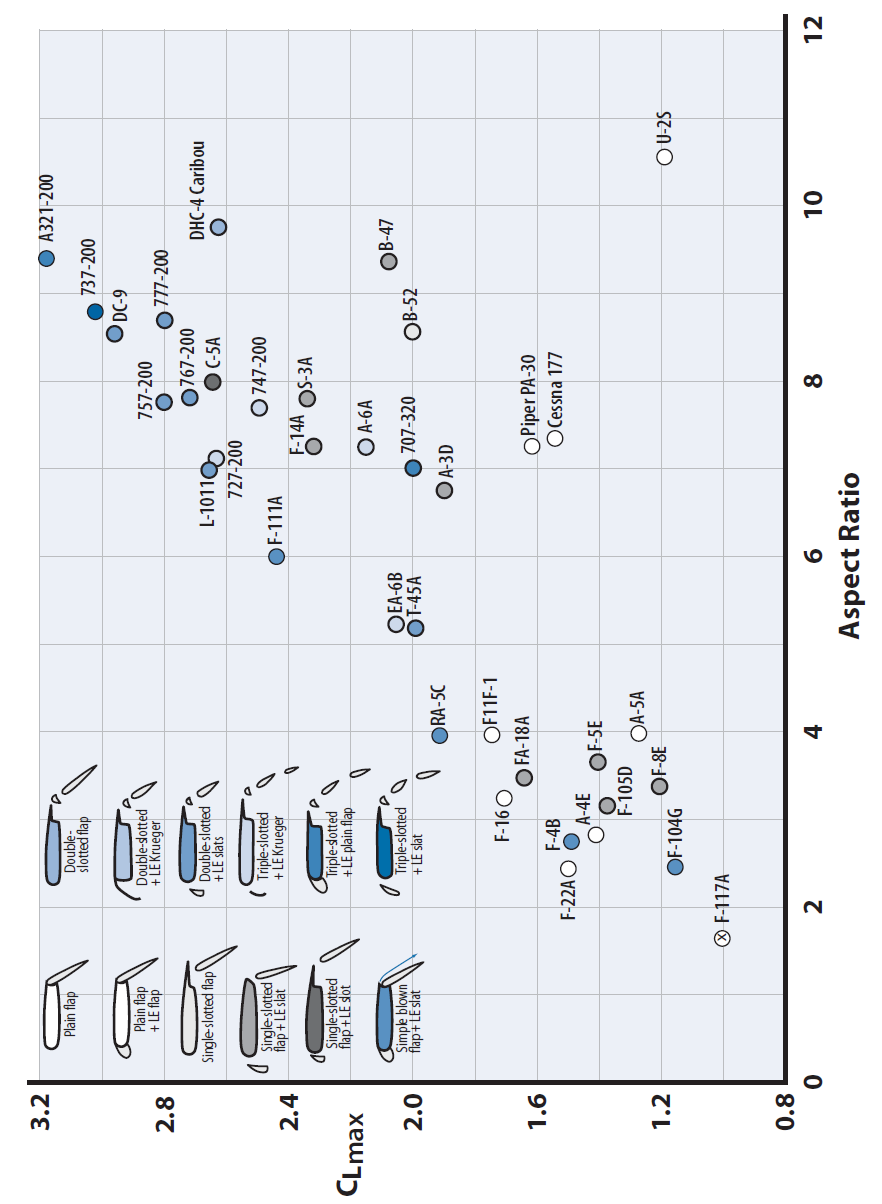
\includegraphics[height=11.3cm, angle =-90 ]{Immagini/highlift.png}} 
\caption{Different kind of High Lift devices and their effects.}
\label{fig:hl}
\end{figure}

In order to evaluate the new wing lift curve with flap and slat it's necessaty to evaluate the contribution due to these devices starting from the clean $C_L$ vs $\alpha$ curve. In particular these contribution on the lift curve are the following:

\begin{itemize}
\item $\upDelta C_{L_0} $ flap 
\item $\upDelta C_{L_{MAX}} $ flap
\item $CL_{\alpha}$ flap 
\item $\upDelta \alpha_{MAX} $ flap
\item $\upDelta C_{L_{MAX}} $ slat
\item $\upDelta \alpha_{MAX} $ slat
\end{itemize}


All of these parameters are calculated using formulas or graphs. For further details see \cite{nicolai2010fundamentals}

\begin{figure}[H]
\centering
{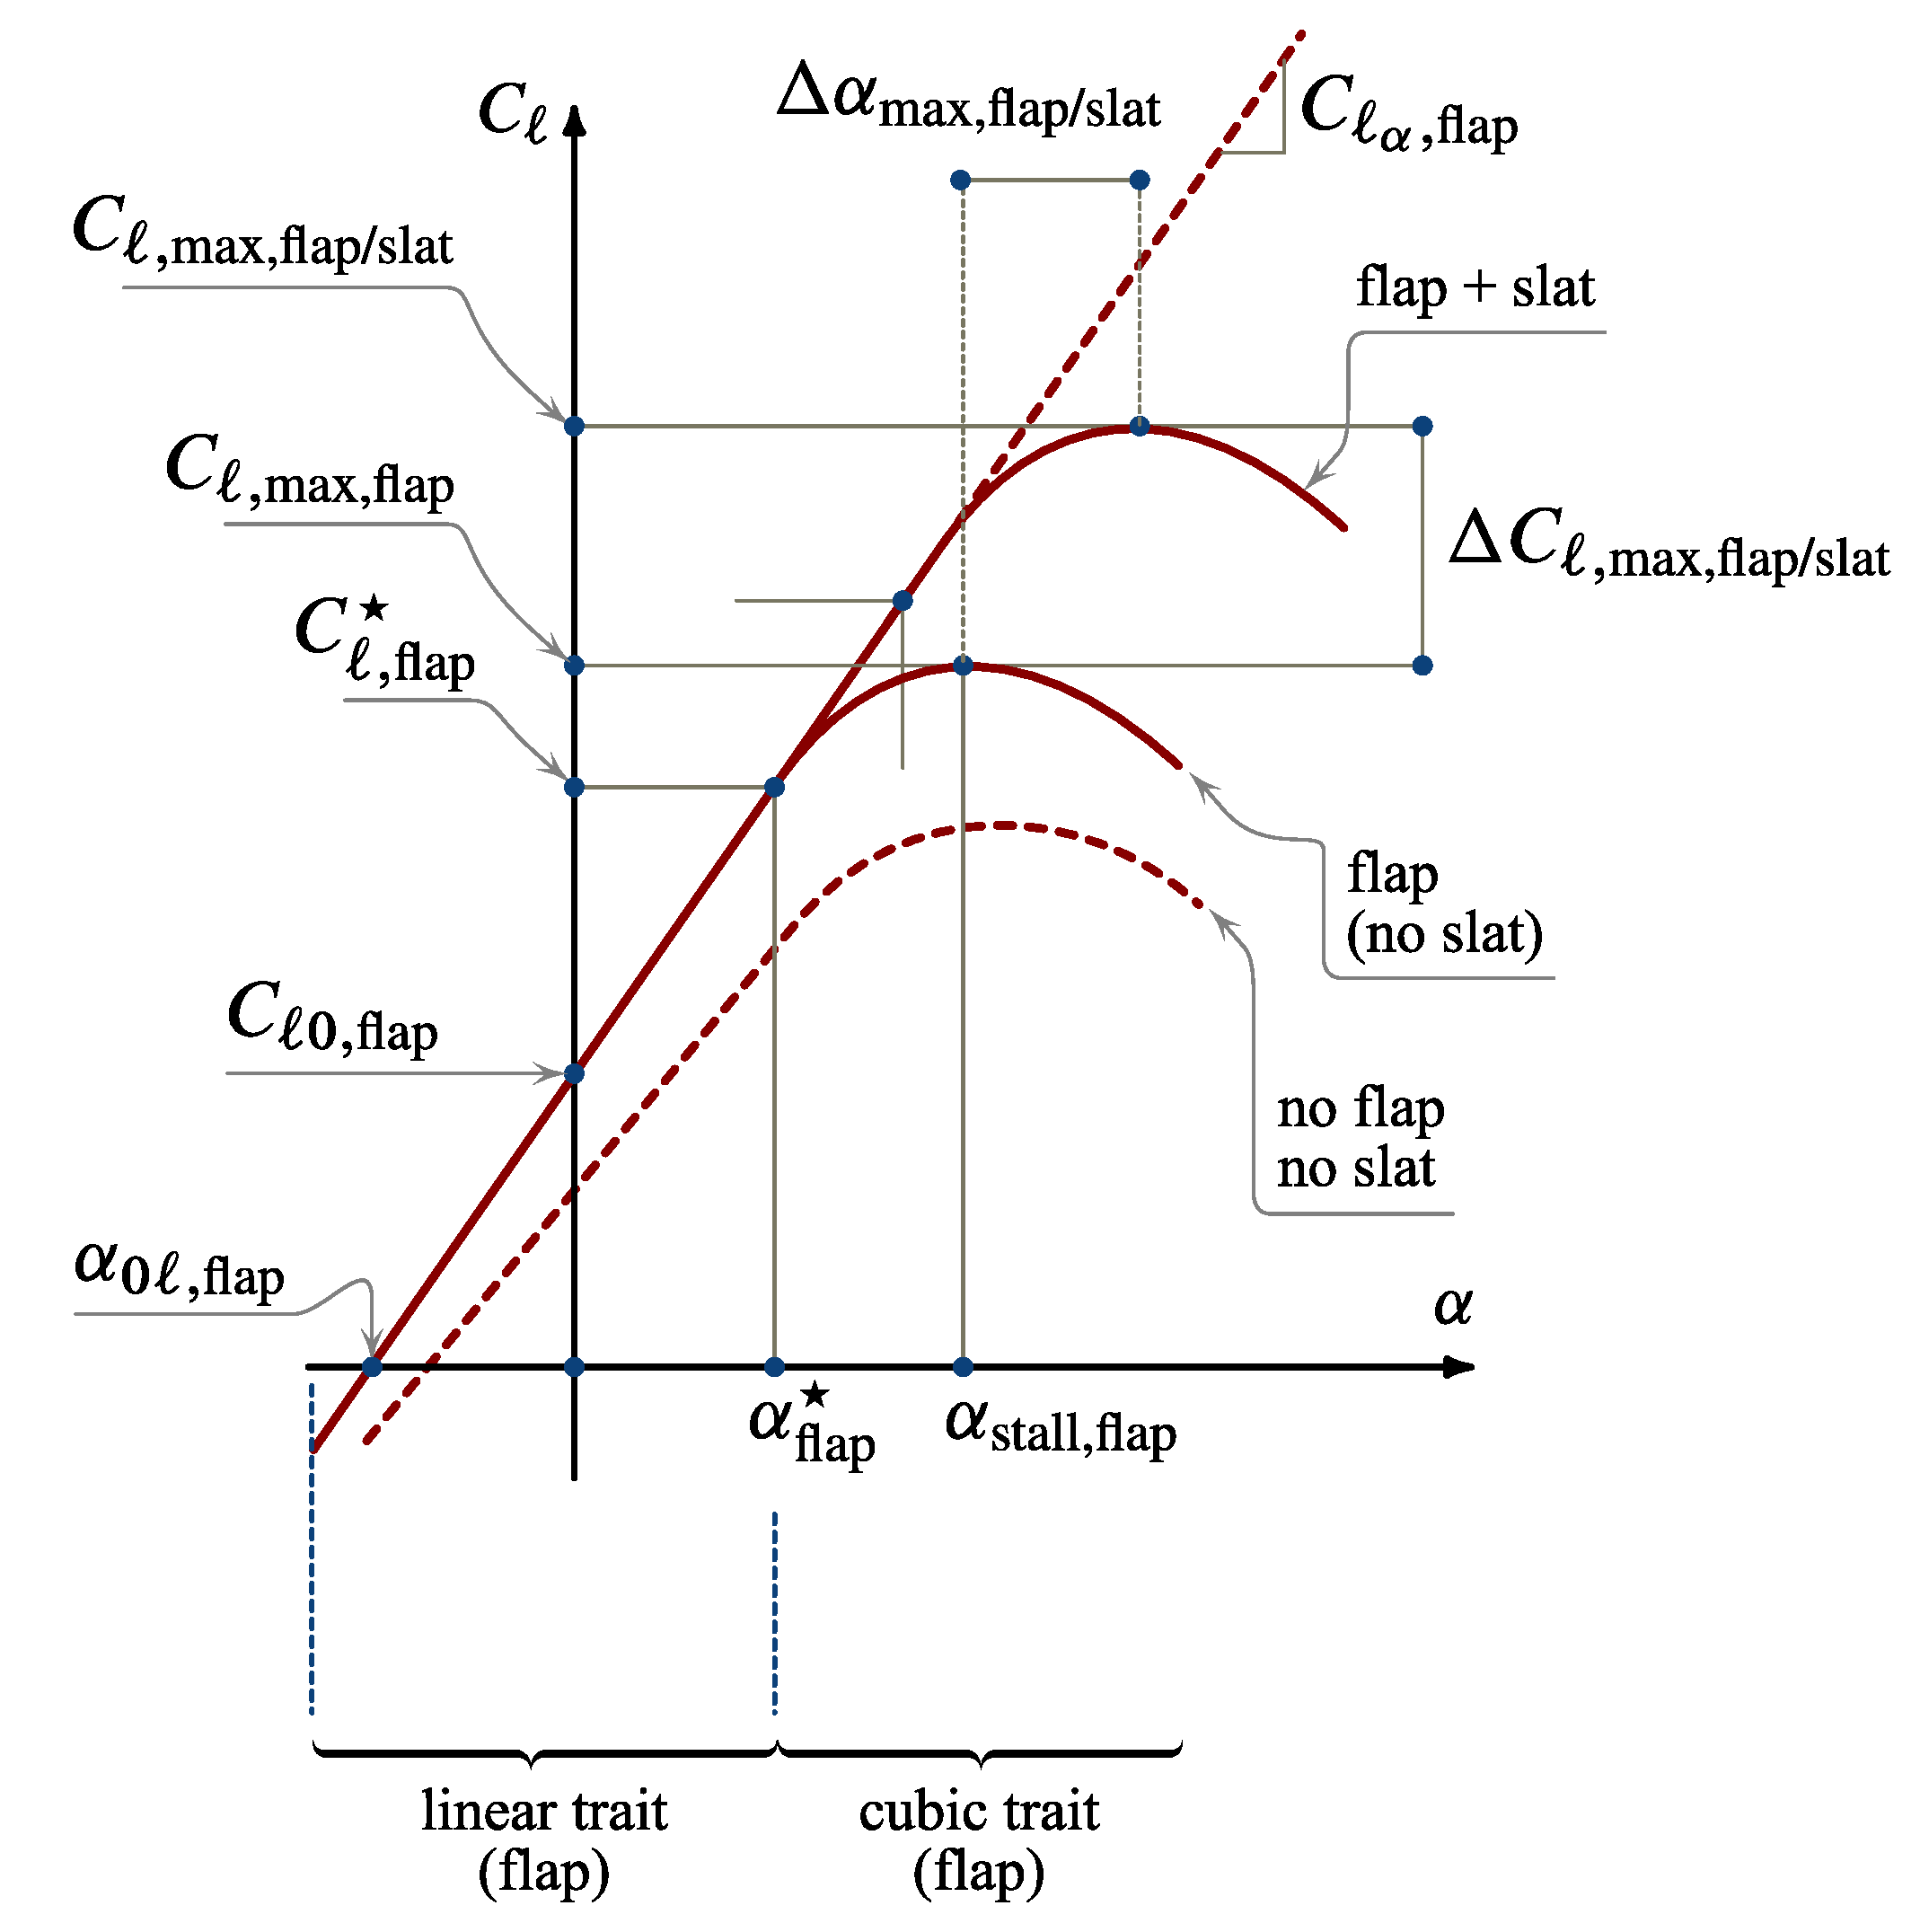
\includegraphics[height=12cm]{Immagini/Airfoil_Cl_Vs_alpha_curve_flap_slat.pdf}} 
\caption{Wing $C_L$ vs $\alpha$ curve for clean wing and with high lift devices.}
\label{fig:clalfahl}
\end{figure}


\section{Java Class Architecture}


%schema con varie classi

\section{Case Study}
%caso di studio
% metti variabilita del cl con mach